\documentclass[10pt]{beamer}

% Packages
\usepackage{graphicx}
\usepackage{hyperref}
\usepackage{listings}
\usepackage{color}
\usepackage{tikz}
\usepackage{amsmath}
\usepackage{amssymb}
\usepackage{helvet} 
\usepackage{caption}
\usepackage{bookmark}

\usetikzlibrary{positioning}

% Beamer settings
\usetheme{metropolis}
\usecolortheme{default}

% Document settings
\title{TFE25-462: Meeting 6}
\subtitle{USRP-GNU Radio Integration and Schmidl and Cox Synchronization}
\author{Quentin Prieels}
\date{\today}


\begin{document}

% Title slide
\maketitle

% Table of contents
%\begin{frame}
%\frametitle{Table of contents}
%    \tableofcontents
%\end{frame}

%%%%%%%%%%%%%%%%%%%%%%%%%%
% PART 1: USRP-GNU Radio %
%%%%%%%%%%%%%%%%%%%%%%%%%%
\section{USRP and GNU Radio}



%%%%%%%%%%%%%%%%%%%%%%%%%%%
% PART 2: Schmidl and Cox %
%%%%%%%%%%%%%%%%%%%%%%%%%%%
\section{Schmidl and Cox Synchronization}

\begin{frame}
    \frametitle{Schmidl and Cox frame structure}
    \begin{itemize}
        \item Require a specific frame structure.
        \item The \textit{preamble} is will have good auto-correlation properties.
        \item It is composed of a single OFDM symbol with data (noise generated) only on even frequencies and zeros on odd frequencies.
        \item This makes the preamble \textit{2-periodic} in time domain.
    \end{itemize}
    \begin{figure}
        \centering
        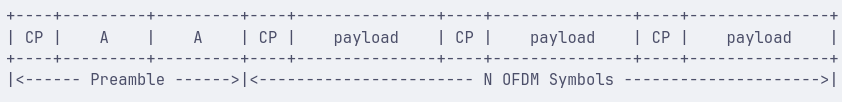
\includegraphics[width=\textwidth]{frame-structure.png}
        \caption{Schmidl and Cox frame structure}
    \end{figure}
\end{frame}

\begin{frame}
    \frametitle{Frame in simulation}
    \begin{figure}
        \centering
        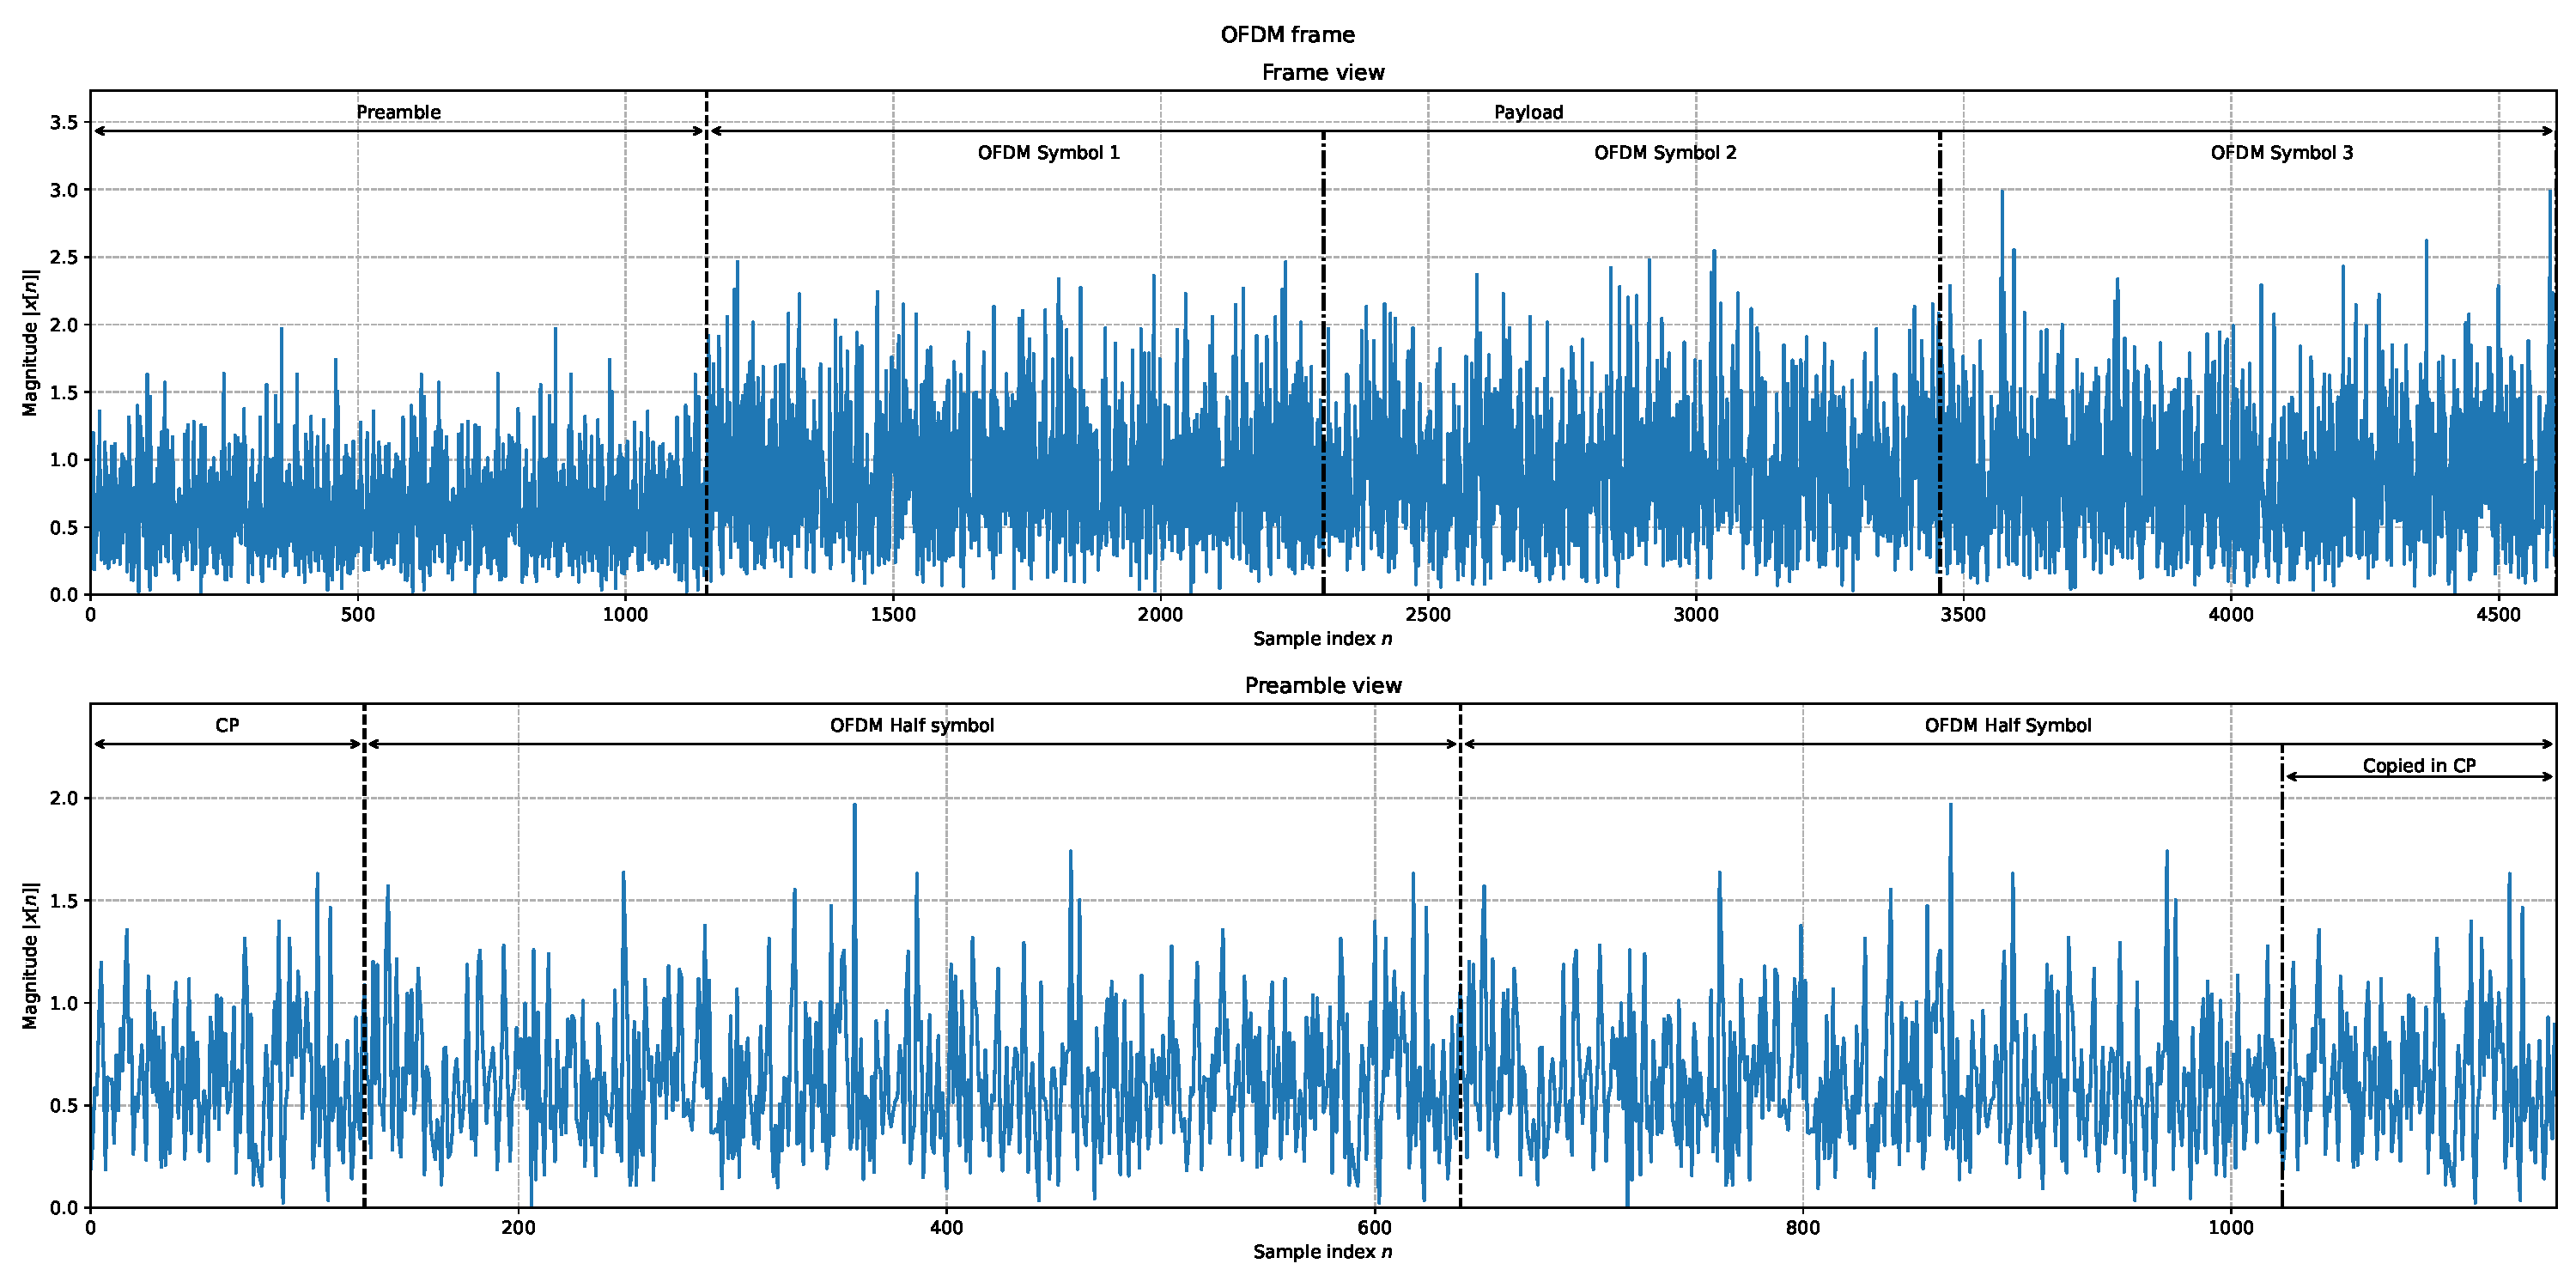
\includegraphics[width=\textwidth]{schmidl_cox_plots/OFDM_frame.pdf}
        \caption{OFDM frame in time domain}
    \end{figure}    
\end{frame}

\begin{frame}
    \frametitle{Time metric $M(d)$ definition}
    In the original paper, Schmidl and Cox proposed to compute the time metric $M(d)$ as follows:
    \begin{equation}
        M(d) = \frac{|P(d)|^2}{(R(d))^2}
    \end{equation}
    with:
    \begin{equation}
        P(d) = \sum_{m=0}^{L-1} r^*(d+m) \cdot r(d+m+L)
    \end{equation}
    \begin{equation}
        R(d) = \sum_{m=0}^{L-1} |r(d+m+L)|^2
    \end{equation}
    where $r(d)$ is the received signal and $L$ is the length of the $A$ symbol in the preamble. With $K$ the number of subcarriers, $L = K/2$, an OFDM symbol in time domain is $K + CP$ samples long.
\end{frame}

\begin{frame}
    \frametitle{Time metric $M(d)$ computation}
    To compute those metrics, Schmidl and Cox proposed to use the following recursive formulas:
    \begin{equation}
        P(d+1) = P(d) + r^*(d+L) \cdot r(d+2L) - r^*(d) \cdot r(d+L)
    \end{equation}
    \begin{equation}
        R(d+1) = R(d) + |r(d+2L)|^2 - |r(d+L)|^2
    \end{equation}

    Remarks:
    \begin{enumerate}
        \item We still need to compute $P(0)$ and $R(0)$.
        \item The system is not causal, still in needs to know the future.
    \end{enumerate}    
\end{frame}

\begin{frame}
    \frametitle{Time metric $M(d)$ in simulation}
    \begin{figure}
        \centering
        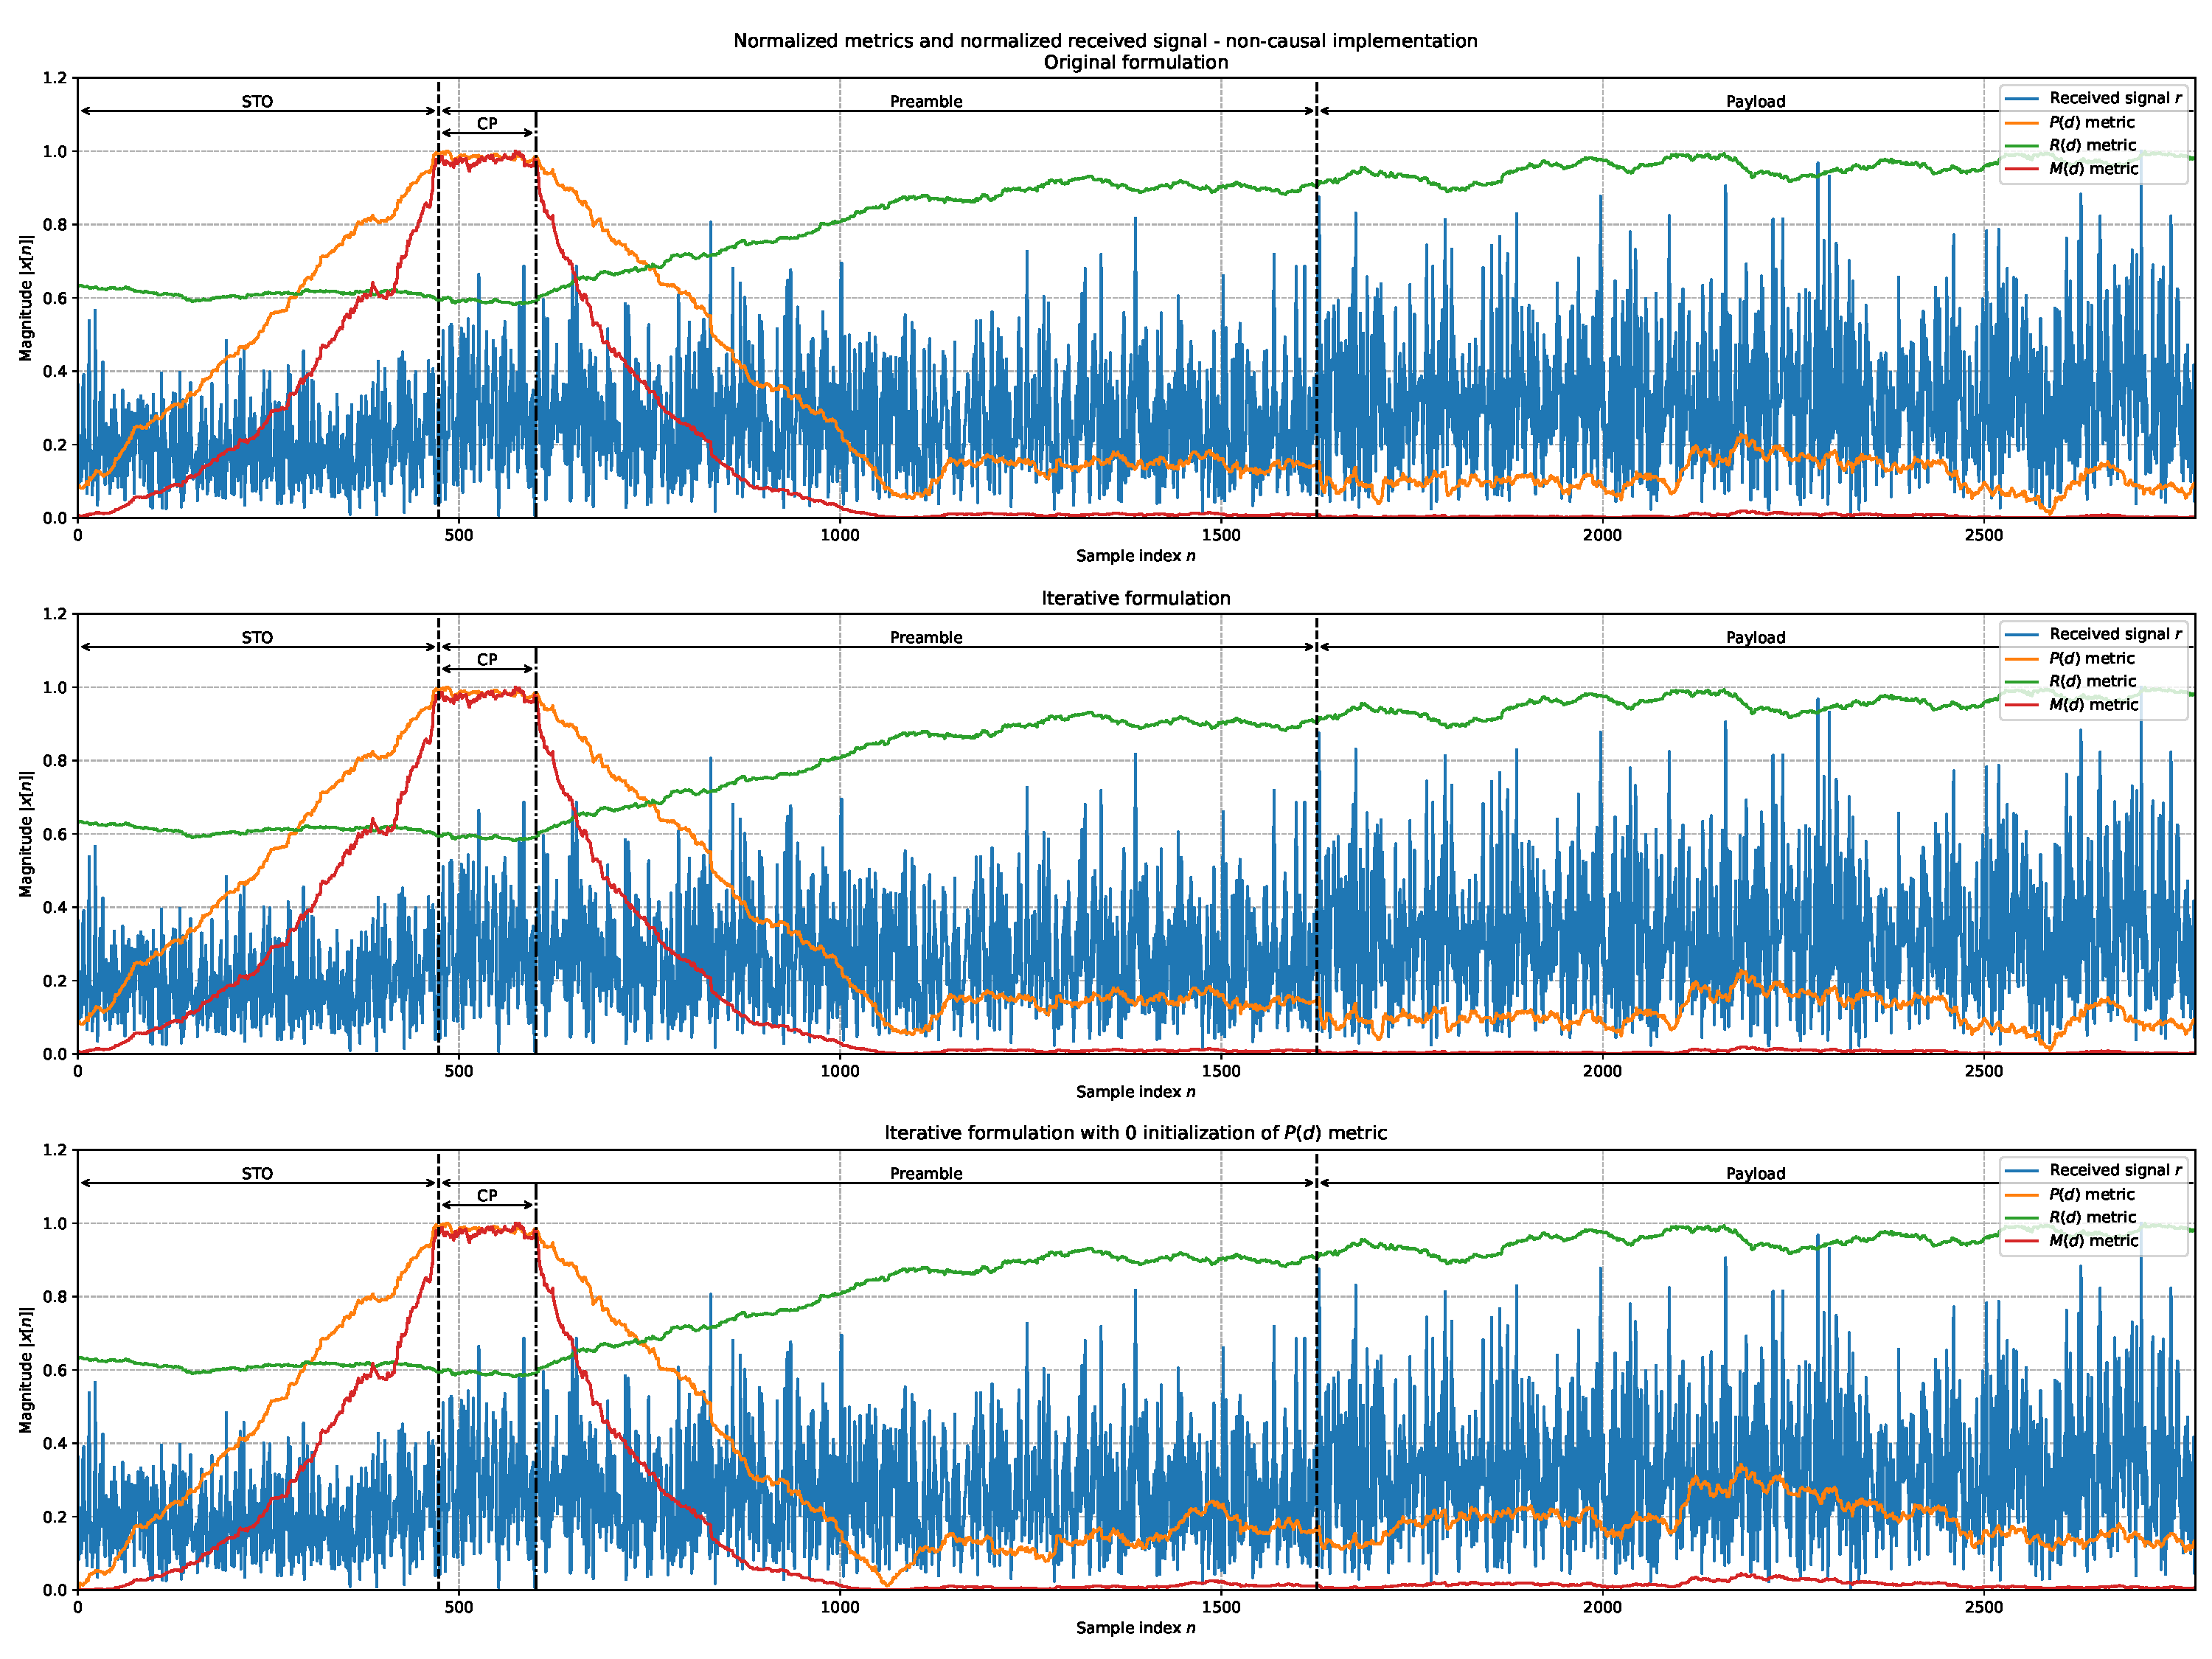
\includegraphics[width=\textwidth]{schmidl_cox_plots/metrics.pdf}
        \caption{Time metric $M(d)$ computation}
    \end{figure}
\end{frame}

\begin{frame}
    \frametitle{Causal implementation of the time metric $M(d)$}
    To make the system causal, we delay the computation of $P(d)$ and $R(d)$ by $2L = K$ samples (length of the OFDM symbol without the cyclic prefix).
    \begin{equation}
        \label{eq:P_causal}
        P(d+1) = P(d) + r^*(d-L) \cdot r(d) - r^*(d-2L) \cdot r(d-L)
    \end{equation}
    \begin{equation}
        \label{eq:R_causal}
        R(d+1) = R(d) + |r(d)|^2 - |r(d - L)|^2
    \end{equation}
    where $R(0)$ is computed as:
    \begin{equation}
        R(d = 0) = \sum_{m=-2L + 1}^{L} |r(m)|^2
    \end{equation}
\end{frame}

\begin{frame}
    \frametitle{Causal implementation using IIR filters}
    By introducing the $v(d)$ signal as $v(d) = r^*(d-L) \cdot r(d)$, we can rewrite the recursive formula as:
    \begin{equation}
        P(d+1) = P(d) + v(d) - v(d-L)
    \end{equation}
\end{frame}

\begin{frame}
    \frametitle{Causal implementation simulation}
    \begin{figure}
        \centering
        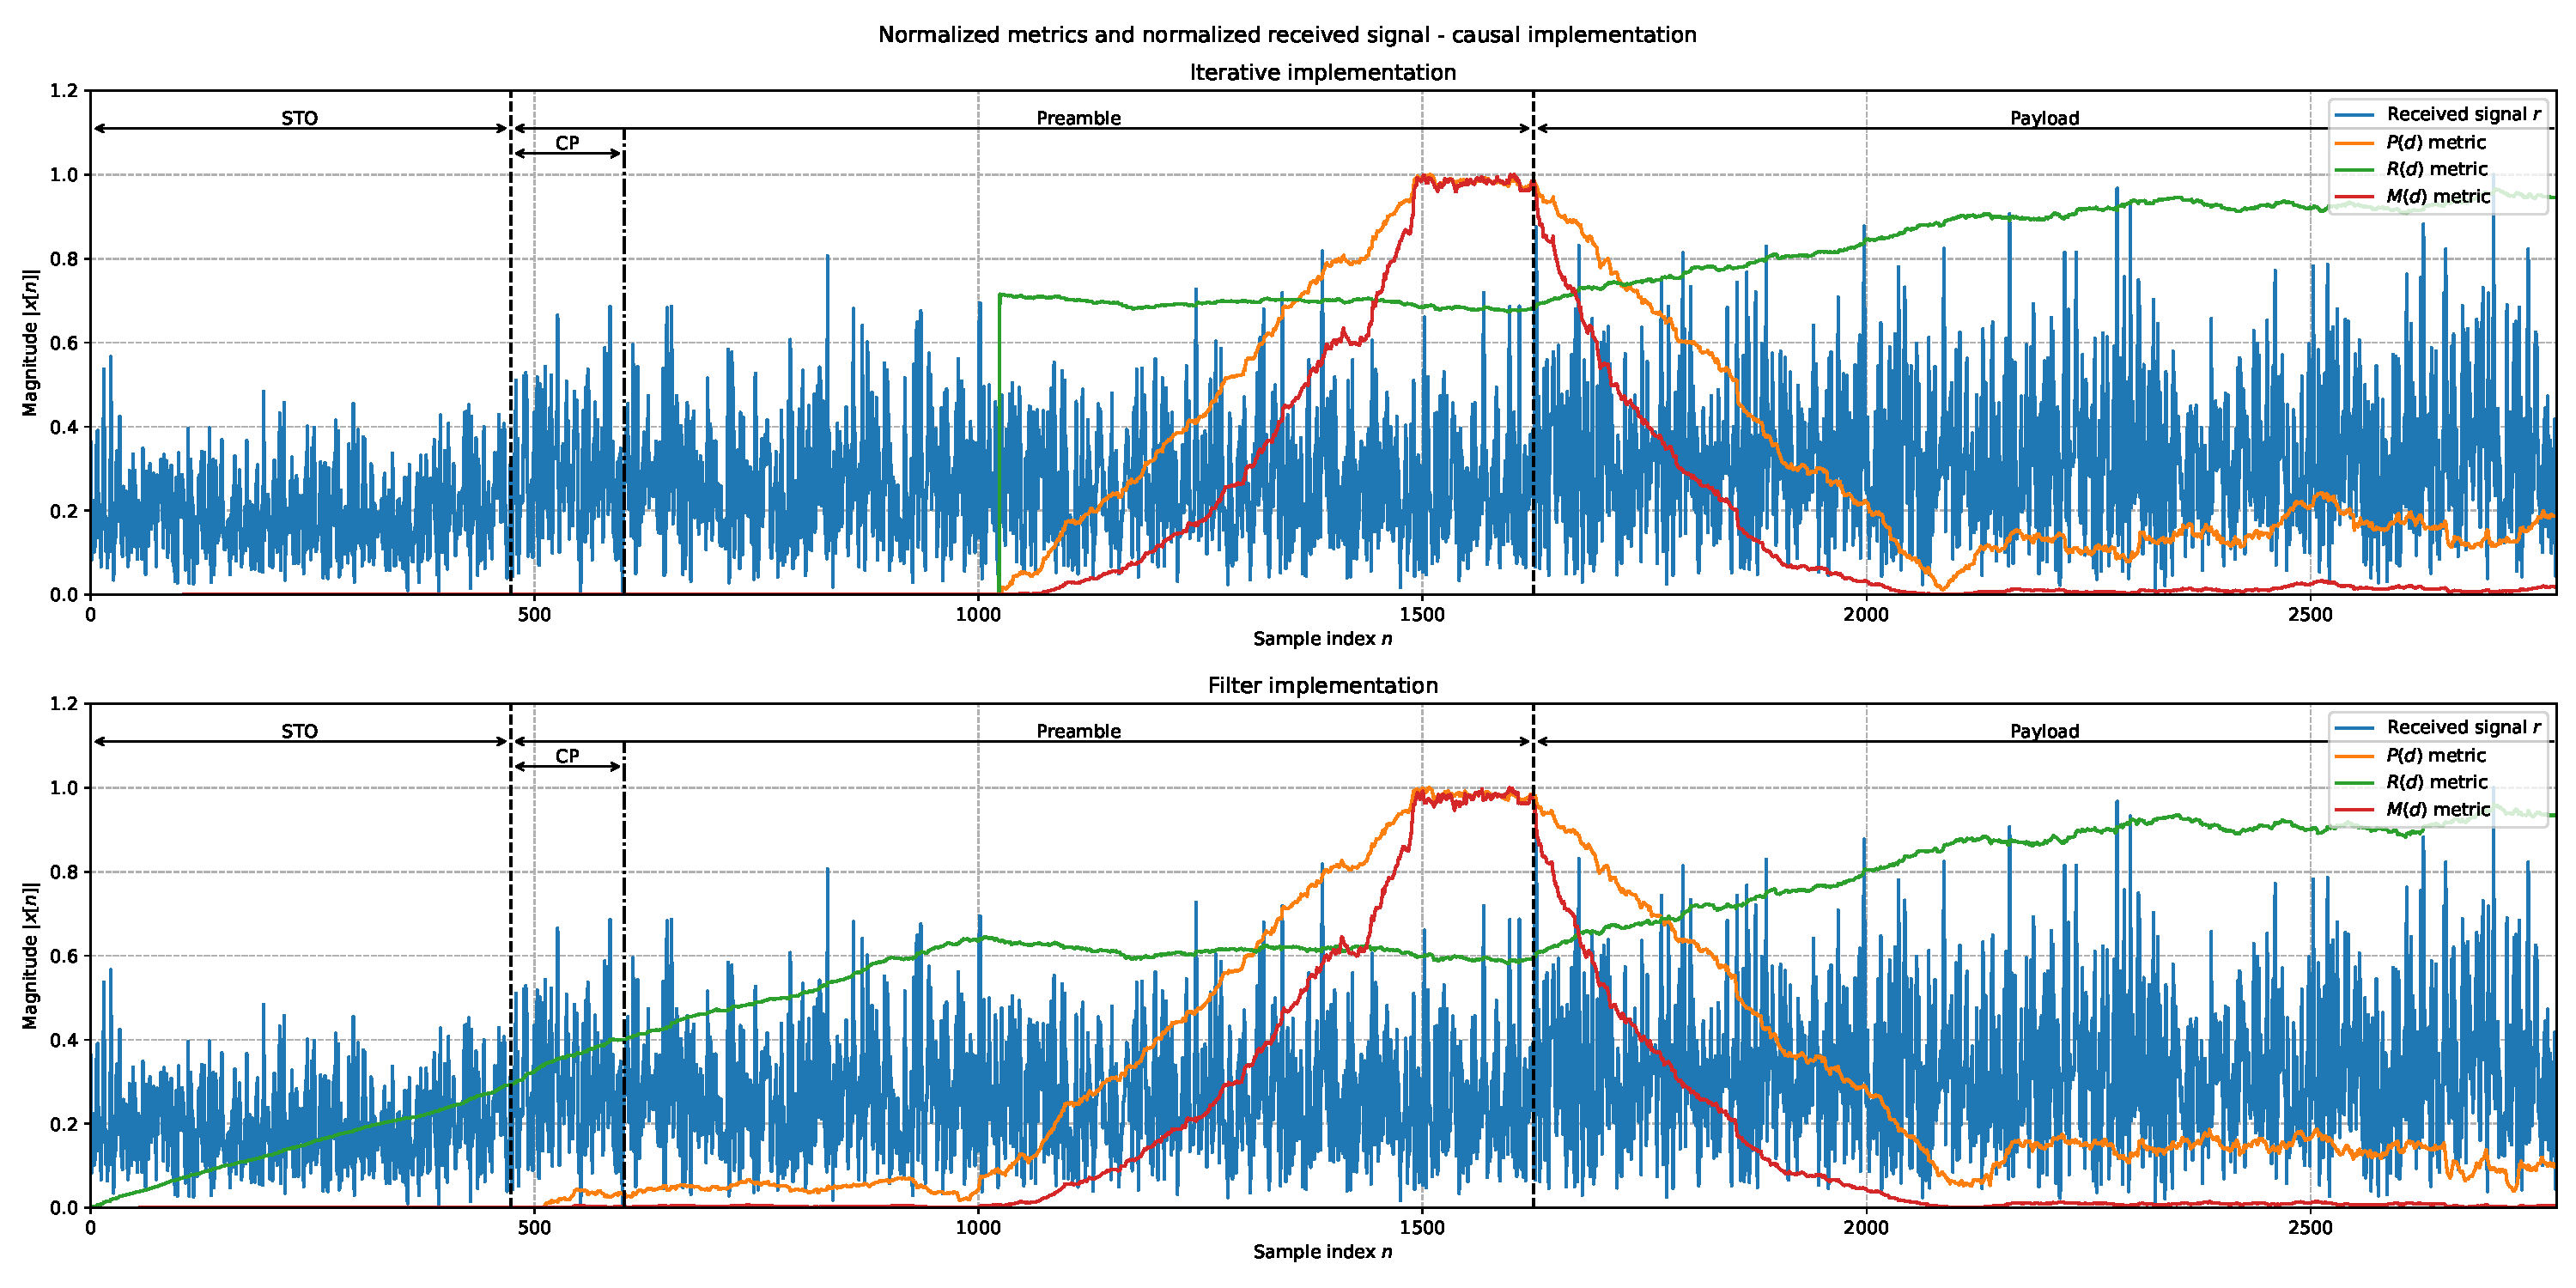
\includegraphics[width=\textwidth]{schmidl_cox_plots/metrics_causal.pdf}
        \caption{Time metric $M(d)$ computation with causal implementation}
    \end{figure}
\end{frame}

\begin{frame}
    \frametitle{If we allow an initialization period}
    If we allow an initialization period of at least $2L$ samples, we can compute the time metric $M(d)$ with equation \ref{eq:P_causal} and \ref{eq:R_causal} without having to compute the "$0$" point.

    \begin{figure}
        \centering
        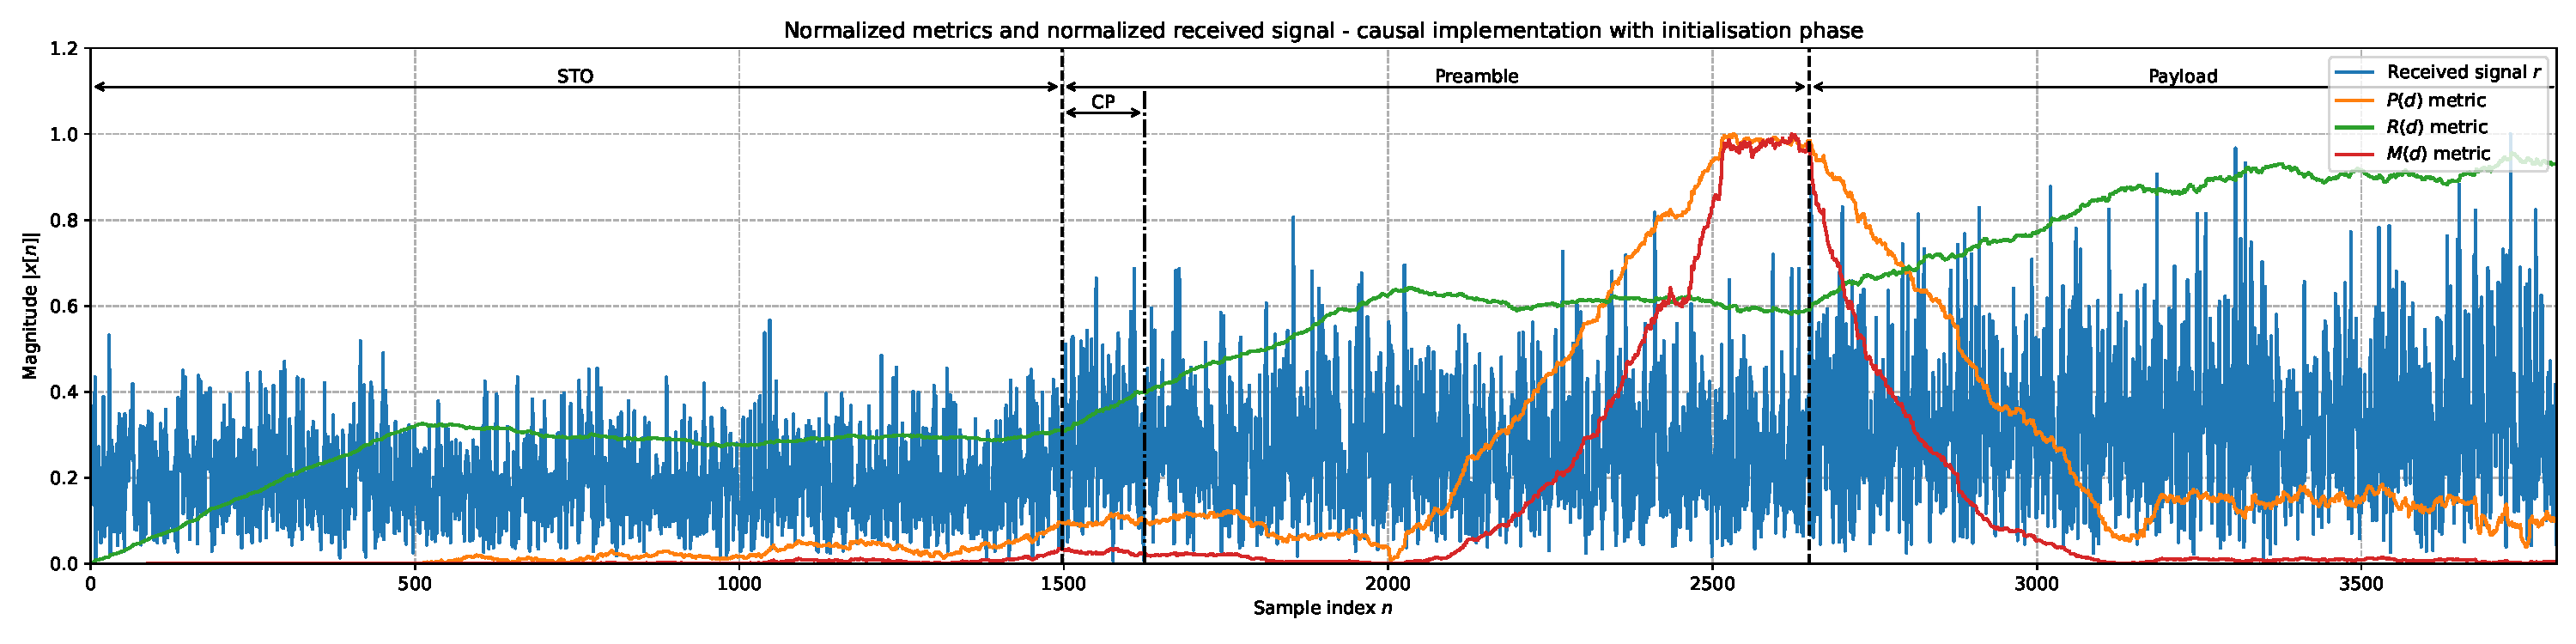
\includegraphics[width=\textwidth]{schmidl_cox_plots/metrics_causal_initialisation.pdf}
        \caption{Time metric $M(d)$ computation with causal implementation and initialization period}      
    \end{figure}
\end{frame}

\begin{frame}
    \frametitle{Time metric $M(d)$ thresholding}
    The time metric $M(d)$ is thresholded to detect the beginning of the frame.
    \begin{figure}
        \centering
        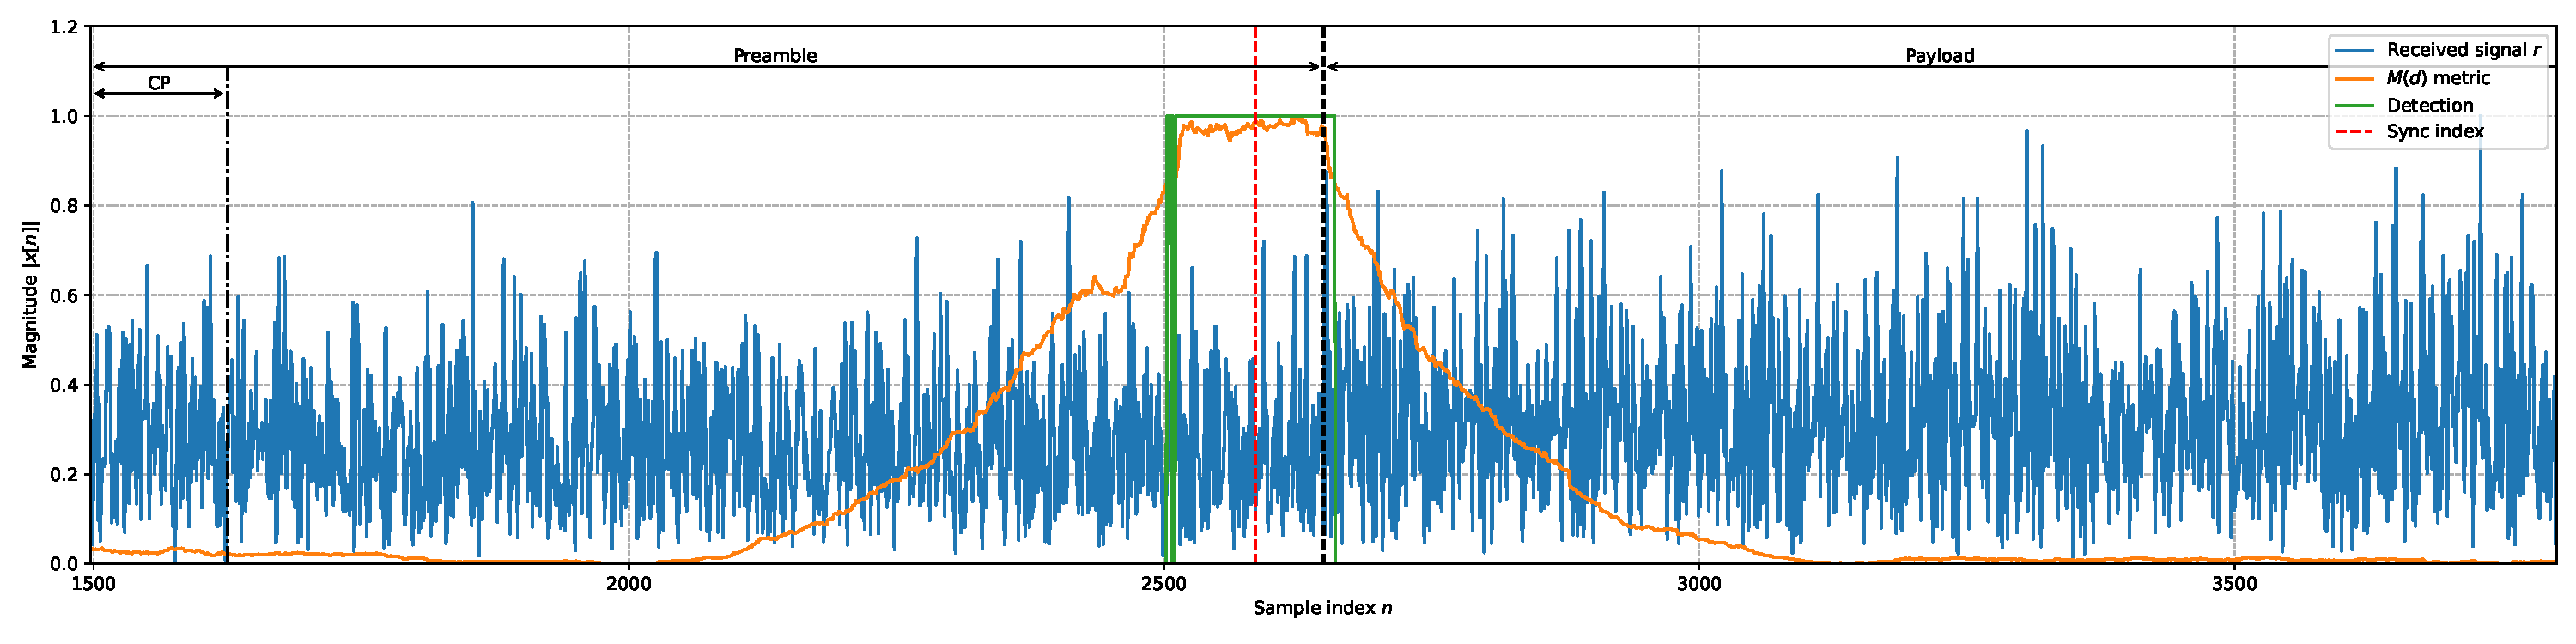
\includegraphics[width=\textwidth]{schmidl_cox_plots/detection.pdf}
        \caption{Time metric $M(d)$ thresholding}
    \end{figure}
    Remarks:
    \begin{enumerate}
        \item How to have a good threshold? (Here it is normalized to the maximum value, how to do it in practice?)
        \item The plateau should be at least $CP$ samples long. We can use this avoiding false positives.
    \end{enumerate}
\end{frame}

\begin{frame}
    \frametitle{Time metric $M(d)$ estimation}
    The value of the plateau depends on the noise power.
    \begin{figure}
        \centering
        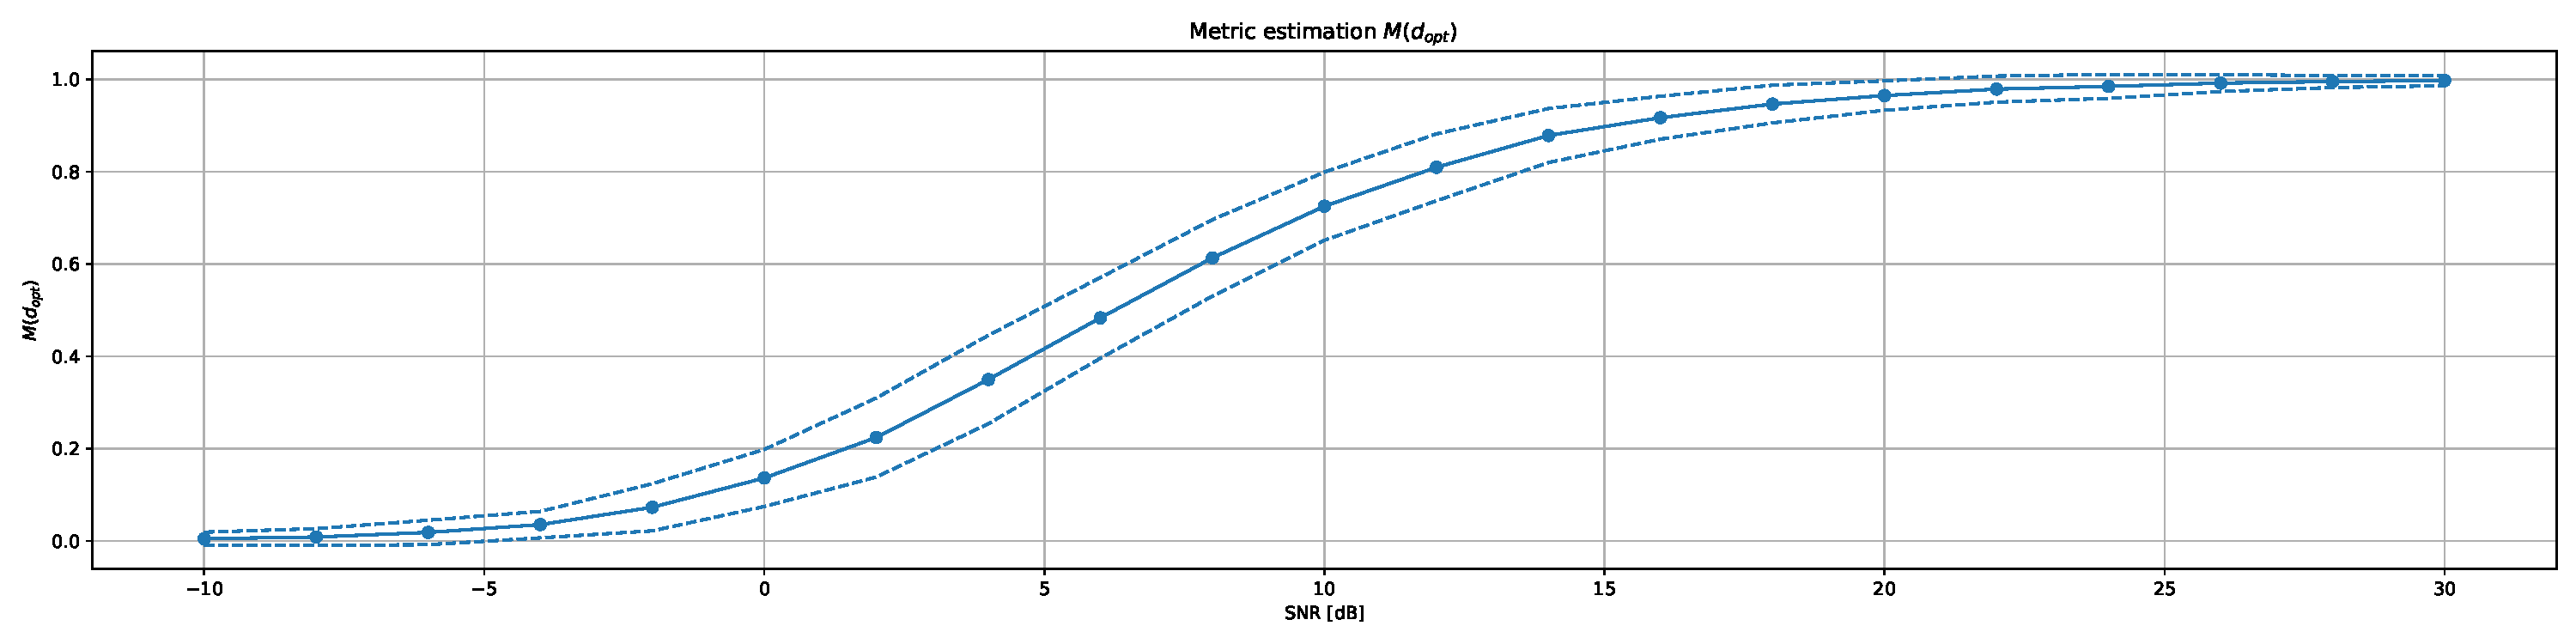
\includegraphics[width=\textwidth]{schmidl_cox_plots/metric_estimation.pdf}
        \caption{Time metric $M(d = d_{opt})$ for different SNRs values}
    \end{figure}
    where $d_{opt}$ is the theoretical beginning of the plateau at \textit{STO + CP + K - CP}. 
\end{frame}

%%%%%%%%%%%%%%%%%%%%%%%%%%%%
% PART 3: Doctorate thesis %
%%%%%%%%%%%%%%%%%%%%%%%%%%%%


\end{document}